\documentclass[10pt,sigconf,letterpaper,anonymous,nonacm]{acmart}

\usepackage{amsfonts}
\usepackage{graphicx}
\usepackage{tikz}
\usepackage{tikzscale}
\usetikzlibrary{positioning}
\usetikzlibrary{shapes.multipart}
\usetikzlibrary{trees}


\graphicspath{ {./graph/} }

\title{Tempus: Probabilistic Network Latency Verifier}
\author{WIP}

\begin{document}
% \shorthandoff{=}
\begin{abstract}
    To combat problems and bugs that a given network might have, network verifiers have emerged as 
    one of the promising solutions. 
    State-of-the-art network verifiers mainly focused on evaluating qualitative properties under 
    various scenarios of network failures, such as reachability under k-link failure. 
    However, as modern networks evolved and performance need becomes more stringent -- often 
    expressed in terms of Service Level Agreement (SLA) -- there is a need to evolve network 
    verifiers to also reason about quantitative performance properties. 
    Works in quantitative network verifiers that has arose in recent years mainly focused on one 
    side of the network performance metric: bandwidth and load violation properties. 
    Questions about the other side of network performance metric, latency, were left unanswered. 

    In this work, we introduce a verifier framework, Tempus, that can answer the probability of 
    a given temporal property being true given latency distributions of individual links and 
    nodes in the network. 
    Early evaluation shows that Tempus can verify bounded reachability property -- the probability
    that the average delay of packets traversing from a source to destination node is below $T$
    time unit -- by only adding a fraction of the state exploration overhead introduced by the 
    qualitative verifier it's built upon.
\end{abstract}

\maketitle



\section{Introduction}
Modern networks consisted of various distributed protocols such as OSPF and BGP that exchange 
routing information so that a packet can reach their intended destination efficiently, even in the 
event of a component failure.
Due to their configuration intricacies however, these protocols are notoriously hard to get right. 
It is hard for a network engineer to reason about whether their configured network fulfilled some 
intended property in various possible states of the network. 
Thus, they are left between the choice of accepting the reality of Murphy's Law or getting a tool 
to help them in this task, namely, network control plane verifier.

Popular control plane verifiers, like ARC \cite{gember2016fast}, are formulated to answer 
questions about a given property deterministically. 
In other words, given a set of states of the network (e.g. $k$-link failures) the verifier are 
expected to give a yes or no answer about the property (e.g. two nodes are reachable).
While useful to some extent, this kind of models are sometimes too restrictive since network 
operators are usually able to tolerate small fraction of failure. 
For example, a given network might have an availability SLA of 99.999\%. 
This kind of probabilistic properties have been the focus of a more recent works like NetDice 
\cite{steffen2020probabilistic}.

The network property itself can also be divided into two kinds. 
Quantitative properties like reachability and loop existence, are the common properties that are 
studied by most of the existing verifiers. 
More recent work, like QARC \cite{subramanian2020detecting}, has also explored qualitative 
properties like link bandwidth violation for a given traffic.

In this work, we're exploring the other side of the network performance metric: latency. 
Certain network deployment often necessitates some latency requirement such as an ISP that has 
latency SLA \cite{Verizon} or deployments of Time-Sensitive Networking (TSN) \cite{TSN}.
We proposed a verification framework to probabilistically verify the latency property of packets 
traversing from a source to destination node under various failure scenarios, by using latency 
information of each components in the network.

\section{Overview}
% \section{On Latency Modeling}
\subsection{Latency as Path Property} 
We began our study by first pondering about a basic construct: modeling the end-to-end latency of 
a single packet.
In a packet-switched network, a packet is sent from one transmiting host to one receiving host 
through the many components of the network (e.g. links, routers, firewall) and each of those 
components might introduce some latency into the packet transmission process.
Figuring out which of those components will actually introduce latency into the packet in question, 
and by how much, is the next logical step that we must figure out.

Obviously, a given packet doesn't need to visit all network components to reach its destination 
host.
A network engineer will configure the network in such a way that a packet will only need to be 
routed via a specific subset of its components.
That specific subset is dictated by two things: how those components are connected together 
(i.e. topology) and how the control plane protocols are configured to route a packet (e.g. routing 
protocol, ACL).
Based on a variety of these setups, nodes in the network will form a forwarding table to route a 
given packet appropriately.

The goal of a classical control plane verifier then, is to use this forwarding table in some 
form to verify certain properties. %TODO: examples?
However, looking at the forwarding table alone will not give us a conclusive result regarding 
which components are going to be visited by a given packet, making verification of latency 
properties less clear.
For example, the network might be configured with a load-balancing protocol in which a packet 
departing from a source host might take multiple different \textit{paths} (with certain 
probability weights) to arrive at the destination host, possibly resulting in a different 
end-to-end latency measurement.

Therefore, we argue that when it comes to analyzing end-to-end latency, a network path should be 
the primary unit of reasoning, rather than forwarding table.
By being more specific about our unit of reasoning, we could answer verification questions more 
clearly, and we could design our verifier more efficiently since we could use it to represent 
multiple different forwarding tables that shares the same path.

\subsection{Relation to Classical Verifier}
Before we analyze the latency of a given packet that propagates through a certain network 
path however, we must make sure that said path exists in the first place.
We note that latency is a property that only make sense after connectivity between two hosts 
has been established. 
In other words, if two nodes in a network aren't even functionally connected (e.g. physical 
link failure, ACL policy), then the latency between them will \textit{always} be infinite, 
making the verification task trivial.

Fortunately, there are a rich body of work in the network verification literature regarding 
functional reachability under failure. %TODO: cite
We could then design our verifier on top of an existing classical control plane verifier.
We use it to verify reachability property, and only if the reachability property is fulfilled, 
we would verify whether the latency between two hosts fulfilled some additional condition.

\subsection{Path Latency Distribution}
Up to this point, we have talked about measuring the latency of a single packet by figuring out 
its path; analyzing which exact components it has traversed through.
However, when we try to generalize this framework and ask questions about the latency of multiple 
packets, it is apparent that the path alone is not a determinative information, as the latency 
of two packets propagating through the same path might be different due to a multitude of factors.

The natural extension to the framework then, is instead of representing latency of a path with a 
single number, we instead represent it with a continuous random variable that signifies the 
possible delay that a given packet traversing through that path might have.
This random variable will have a distribution that marginalizes over all other factors other than 
the path.

We can then use this latency distribution to verify some temporal properties in a probabilistic 
manner.
For example, we could verify the probability that a packet will be delivered in under a time 
unit by taking the CDF of the distribution.

\subsection{Path Decomposition and Convolution} \label{decomposition}
The final question that we had to decide on was how do we actually model path latency distribution
based on real component measurements.
Considering the complexity of factors that might determine the path latency distribution and the 
availability of measurement data, we settle on the assumption that the path latency distribution 
is composed of multiple independent distribution that corresponds to the latency each components 
in the path might introduce.
%TODO: confirm about independence?

Since not all components in the path will introduce latency with a non-negligible value, we 
specifically choose to model two source of latency in the path's components which we deem 
significant: \textbf{link propagation latency} and \textbf{queuing latency}.
%TODO: expand on how to get the data later

Propagation delay is the latency that is introduced by the links in the network, which is 
independent of the traffic load in the system.
Queuing delay is the latency that the queuing process in the node introduced. 
Unlike propagation delay, queuing delay might be dependent on load in the system, since the more 
packets there are in the queue, the more delay the node will introduce to a subsequent packets.

For propagation delay, the semantic of this random variable is relatively straightforward: it is 
the distribution of latency that a given link will introduce.
For queuing delay however, this random variable represents the delay that a given queuing process 
will introduce, marginalized over various traffic pattern that a given network state might have 
resulted.

In order to obtain the overall path latency distribution from these per-component latency 
distributions, we do a convolution operations over all the relevant component's latency 
distributions.
Since not all distributions can be convolved in a closed-form fashion, we use a numerical 
convolution technique with a guaranteed error bound. 
We initially consider a Monte-Carlo simulation in order to approach numerical convolution, but 
the lack of a general technique to measure error made us opt for the formerly mentioned method.


% \section{Verifier Design}
We divide the problem of latency verification into two parts: 
verifying that two nodes are reachable (\textbf{functional verification}) and only if 
the functional property is fulfilled, we would verify whether the latency between 
two nodes fulfilled some temporal condition (\textbf{temporal verification}).

\section{Functional Verification}
For functional property verification, NetDice \cite{steffen2020probabilistic} 
has laid the way for verifying reachability between two nodes under failure in a 
probabilistic and efficient manner.
To contextualize our modification, we will briefly describe some parts of 
NetDice's network encoding and exploration algorithm as a prelude to our alteration.
For a more complete complete description of NetDice, please refer to the original 
paper.

\begin{figure}[h]
    \centering
    % \includegraphics[width=0.4\textwidth, trim=0cm 11cm 0cm 5cm]{ex.pdf}
    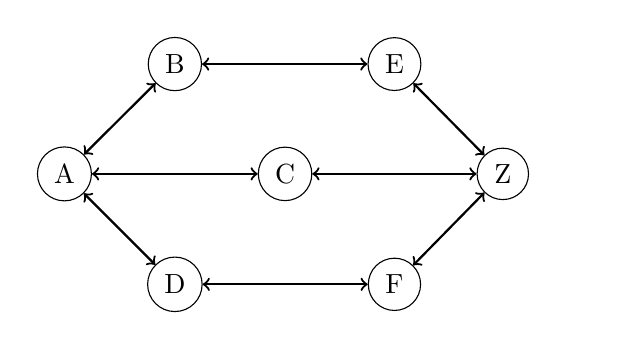
\begin{tikzpicture}
    \matrix[column sep=7mm, row sep=7mm]{
        & \node[draw, shape=circle](B){B}; & & 
        \node[draw, shape=circle](E){E}; & & \\
        \node[draw, shape=circle](A){A}; & & 
        \node[draw, shape=circle](C){C}; & & 
        \node[draw, shape=circle](Z){Z}; \\
        & \node[draw, shape=circle](D){D}; & & 
        \node[draw, shape=circle](F){F}; & & \\
    };
    \draw[<->, thick] (A) -- (C);
    \draw[<->, thick] (C) -- (Z);

    \draw[<->, thick] (A) -- (B);
    \draw[<->, thick] (B) -- (E);
    \draw[<->, thick] (E) -- (Z);

    \draw[<->, thick] (A) -- (D);
    \draw[<->, thick] (D) -- (F);
    \draw[<->, thick] (F) -- (Z);
\end{tikzpicture}
    % \includegraphics{ex.eps}
    \caption{Example topology, we want to check the reachability of A to Z}
    \label{fig:ex}
\end{figure}

\begin{figure}[h]
    \centering
    % \includegraphics[width=0.4\textwidth, trim=0cm 11cm 0cm 5cm]{ex.pdf}
    \includegraphics[width=\columnwidth]{../tikz/tree}
    % \includegraphics{ex.eps}
    \caption{Subset of Modified Exploration Tree, $\mathcal{E}_2$ and $\mathcal{E}_3$ 
        will get consolidated, so does $\mathcal{E}_4$ and $\mathcal{E}_5$}
    \label{fig:tree}
\end{figure}

\subsection{Topology Graph}
In this framework, a network is encoded in an edge-labeled directed graph 
$G_t = (V_t, E_t)$ where $V_t$ represents the nodes in the network and 
$E_t$ represents the functional connectivity between a source and a destination node. 
A physical link is then represented as a pair of symmetrical edges that shares the same source 
and destination node but with opposite direction (e.g. $v_1 \rightarrow v_2$ and $v_2 
\rightarrow v_1$).

% To represent the component's random failure, NetDice defined two failure rates.
% The first failure rate is the chance that a given physical link in the network will go down.
% The second failure rate is the chance that a given node in the network will go down.
% These rates are shared between all links / nodes in the network.
% Internally however, the node failure rate will be translated into the link failure rate 
% with a Bayesian Network model, since a node failure can be modeled with the failure of each 
% links connected to it.

To represent random failure, NetDice defined a universal link failure rate (i.e. 
the probability of \textit{any} link in the network randomly failing).
We refine NetDice's model slightly by allowing each links to have different failure rate.
We label each edge in $E_t$ with a function $r: E_t \rightarrow \{x \in \mathbb{R} \mid 0 \le x 
\le 1\}$ that represents the failure rate of a given physical link.
As a consequence, two symmetrical edges (i.e. two edges that shares the same node pairs but with 
opposite direction) will also share the same failure rate, and will be disabled in a coupled 
fashion.

% \subsubsection{Routing}
% On top of this topology, NetDice also defined additional informations that would be used
% by a routing protocol to determine the valid path(s) between two nodes $src, dst \in V_t$ given 
% a particular link failure scenario. 
% These routing informations would also be used by their optimization algorithms to reduce the 
% amount of states that are going to be explored.

% NetDice implemented iBGP and OSPF (with ECMP) routing protocols.
% They encode the relevant routing information by assigning some labels to the vertices or edges
% in the topology.
% In OSPF for example, we define a function $w_{ospf}: E_t \rightarrow \mathbb{N}$ as the edge-label 
% that represents the positive weight of a link.
% They would later be used to compute the convergent paths of a given network state 
% (\ref{verification}).

\subsection{State Exploration}
A \textbf{network state} is defined as a set of failed links.
There are $2^{|E_t|}$ network states in a given network and a brute-force strategy 
would need to explore all of the states to compute the reachability property of a 
node pair in a given network. 
NetDice however, will merge multiple network states into an \textbf{equivalence class}
by marginalizing over \textit{cold edges}, links whose failure is guaranteed not to 
change the convergent path of a highlighted network state.

NetDice will systematically explore many equivalence classes in the network. 
It will start from the equivalence class of a perfect network and will fail certain 
\textit{hot edges} (i.e. edges that are not cold) to explore another equivalence 
class.
While not explicit in its description, NetDice's algorithm will effectively form an 
\textbf{exploration tree} (Fig. \ref{fig:tree}). 

In order to preserve some information that will be used in the temporal verification 
stage, we modify this original exploration algorithm to make it more explicit.
We started by formalizing the notion of Equivalence Classes.
An Equivalence Class $\mathcal{E}$ is defined as a 3-tuple $(U_h, D_h, P_{conv})$.
$U_h$ and $D_h$ refers to a set of hot edges that are up and down respectively.
$P_{conv}$ refers to the convergent paths between src-dst pair that is produced by the
control plane when the links in $D_h$ fails.
Unlike the original algorithm, we explicitly store $P_{conv}$ in $\mathcal{E}$ so that 
it could be used to for the temporal verification stage.

We then define the Exploration Tree $\mathcal{T}$ as a tree of Equivalence Classes.
At the root, we have an Equivalence Class that corresponds to a perfect network, where 
$P_{conv}$ is the path(s) that the control plane will produce given a perfect network 
condition and $U_h = D_h = \emptyset$.
Each Equivalence Class in this tree will have children which have one of its parent's link in 
$P_{conv}$ appended to its $D_h$, essentially failing one of the link in the path.
If an Equivalence Class has an empty $P_{conv}$, then it would have no children.

To compute the functional probability of a given Equivalence Class, we compute the 
product of the 'up' probability of all the links in $U_h$ and $P_{conv}$ and the 
product of the 'down' probability of all the links in $D_h$.

After having the algorithm produced $\mathcal{T}$, we then continue to the temporal verification 
stage.

\section{Temporal Verification}
In the temporal verification stage, we will use the path information that we got from 
functional verification stage and augment them with latency information to 
produce the final temporal property probability.

\subsection{Latency Label}
Similar to link failure $r$, we use edge-labeling technique to represent latency that 
will get introduced by the connectivity between two nodes. 
Our model will model two significant sources of latency: \textbf{link propagation} 
and \textbf{packet queuing in the node}.
We will encode these latencies by equipping the model with two additional labels.

Encoding link propagation latency is fairly straightforward. 
We define a function $l_p: E_t \rightarrow \mathcal{D}$ where $\mathcal{D}$ is a set of 
continuous univariate distribution that has a minimum value of $0$.
This distribution signifies the time it would take for the respective physical link to transmit 
a packet from one end to another.
Because of this, just like $r$, two symmetrical edges will share the same distribution.

To encode queuing latency, we first note that the queuing mechanism in modern switches 
usually resides in the output port. %TODO: Cite PISA?
Since a port in a switch is only connected to one other port, we could effectively 
assign the latency to the connectivity between switches.
To do this, we define another function $l_q: E_t \rightarrow \mathcal{D}$.
This distribution signifies the output queue latency in the source node that is 
going to be forwarded to the destination node.
Unlike $l_p$, two symmetrical edges will have two different distributions since they 
represent two different output queues.

Given $P_{conv}$, $l_p$, and $l_q$, we could then compute the probability of a given 
temporal property being fulfilled.
We will describe our algorithm for computing this probability in the next few 
sections.

\subsection{Weighted Average and Path Convolution}
Since a convergent behavior of the forwarding plane $P_{conv}$ might contain more than 
one paths, we will compute the temporal probability of $P_{conv}$ by computing the 
weighted average of the temporal probability of each of the individual paths.
The specific weight depends on the load-balancing method used.
We have implemented the weight computation for ECMP load-balancing scheme.

To get the temporal probability of a single path, we will use the latency information 
from $l_p$ and $l_q$ to compute the latency distribution of the whole path.
To do this, we resort to the methods of \textbf{convolution}.
For each edge $e$ in the path, we will get $l_p(e)$ and $l_q(e)$ and convolve them 
all together to get the path latency distribution.

With this path latency distribution, we could get the temporal probability of a 
path by computing the statistical property of said distribution.
In this work, given a path latency distribution $\mathcal{L}$, we define two temporal 
properties:
\begin{itemize}
    \item \textbf{Bounded Reachability}: the probability that a packet will get 
        transmited below $t$ time unit. This will get computed as $cdf(\mathcal{L}, t)$
    \item \textbf{Tail Reachability}: the probability that a packet will get 
        transmited above $t$ time unit. This will get computed as 
        $1 - cdf(\mathcal{L}, t)$
\end{itemize}

In short, given $P_{conv}$, $l_p$, and $l_q$, we will compute:
\begin{enumerate}
    \item Split $P_{conv}$ into its individual path
    \item For each path, compute its latency distribution by convolving the latency distribution 
        $l_p$ and $l_q$ of each link
    \item With the resulting path latency distribution, determine the probability of temporal 
        property by computing the statistical property of said distribution
    \item Combine the temporal property of each path by computing the weighted average, based 
        on the load-balancing scheme of the control plane
\end{enumerate}

We do each of these steps to every Equivalence Class in $\mathcal{T}$, and thus adding additional 
overhead to the exploration algorithm (on top of functional exploration).
In other words, for $\mathcal{T}$ of size $n$, we will need to do temporal verification in each of 
those $n$ Equivalence Class.
We aim to minimize the overhead of temporal verification by introducing some optimization algorithms
later.

% \section{Verification} \label{verification}
% From a labeled graph that encodes a given network, we will then do functional verification 
% and temporal verification in the following way:

% \subsection{Functional Verification}
% For functional verification, we will essentially do the exploration technique employed by NetDice.
% However, we made some modifications to the algorithm in order for it to remember and pass 
% necessary informations to the temporal verification stage.
% To contextualize our modification, we will briefly describe the description of NetDice's algorithm 
% in three parts: Network States, Equivalence Classes, and Functional Exploration.
% For a more complete complete description of NetDice, please refer to the original paper.

% \subsubsection{Network States}
% Let a network state $s_i$ be defined as a 2-tuple $(U, D)$ where $U$ is a set of all links that 
% are alive / up and $D$ is a set of all links that are dead / down.
% (Consequently, $E_t = U \cup D$).
% We then define a set $S$ that represents all possible network states in a given topology. 
% The goal of functional verification is to identify the largest subset of $S$ where each element 
% of this set is a network state that can connect the source and destination node given a convergent 
% behavior of the control plane.
% We will call this subset \textit{reachability subset}.
% While NetDice posseses the ability to verify other properties, we only focuses on basic 
% reachability, the most relevant property for latency verification.

% This framework fits nicely with the framework of probability theory, where $S$ represents the 
% sample space and the power set of $S$ represents the possible probability events, one of which is 
% the previously mentioned reachability subset.
% The way we assign probability values to a subset is to simply do a summation over the probability 
% value of each network state, which in turn is the product of all the failure and success rate of 
% each links in the network state.

% The naive approach to compute the probability of the reachability subset is to exhaustively iterate 
% over all the network state and check the reachability property. 
% While natural, this brute-force algorithm doesn't scale well since it will take 
% $2^{|E_t|}$ iterations. 

% \subsubsection{Equivalence Classes}
% NetDice \cite{steffen2020probabilistic} solves this issue by noticing that we could combine over 
% some states that are guaranteed not to change the convergent paths (and thus the reachability 
% property) of the current network state, by marginalizing over what is called \textit{cold edges}.

% Cold edges are defined to be links whose failure is guaranteed not to change the property in 
% question.
% In the specific case of reachability, this essentially mean that the failure of such edge 
% won't change the convergent paths of the network state in question.
% By marginalizing over its cold edges and combining the state into one equivalence class, instead 
% of computing the probability of individual network states, we are left with computing the 
% probability from the remaining edges, which is called \textit{hot edges}.

% Hot edges are the opposite of cold edges: their state (whether they are up or down) will change 
% the convergent path of the network state in question.
% Mostly, they consists of the links that make up the convergent paths itself.

% By identifying the cold edges of a given network state, NetDice reduces the search-space by 
% merging multiple network states into fewer equivalence classes. 
% However, this optimization also serves another purpose: providing an efficient exploration 
% strategy. 

% \subsubsection{Functional Exploration}
% To actually identify the equivalence classes that might emerge in a given network, NetDice employs
% a tree-based exploration method based on hot edges computation.

% We start with a perfect network state (i.e. $s_i = (U, D)$ where $D = \emptyset$ and $U = E_t$).
% We then compute the convergent paths and determine the hot edges set of that network state.
% Since, by definition, shutting down the link in this set will change the convergent paths, 
% instead of exhaustively exploring some other state at random, NetDice would continue the 
% exploration by systematically failing one of these links instead.

% We then determine whether that network state can fulfill said property and which path it will 
% take, similar to the brute-force method.
% If no, then it is safe to say that the source node can never reach the destination node in all 
% network state.
% If yes, then we could use the logic of the routing protocol to determine the set of cold edges, 
% (i.e. edges whose failure won't change the convergent paths). 
% Edges that are not part of this set is called \textit{hot edges} $h_i = (U, D)$.
% Instead of using $s_i$ to compute the probability of the current state, NetDice only use the set 
% of hot edges to compute the probability of them being alive ($h_i = (U, D)$ where $D = \emptyset$).
% This in effect computes the probability of multiple network state at once.

% Next, instead of examining other network state at random, we instead iterate over the links in 
% $h_i$.
% By definition, if we fail a link that belongs to $h_i$, then the convergent paths will change.
% To cover all of those possibilities efficiently, NetDice iterate over all the links in $h_i$, 
% disabled them, re-enabled them, and move to the next edge to do the same.
% If $h_i = ((e_1, e_2, ..., e_j), \emptyset)$, then we would enqueue $(\emptyset, (e_1))$, 
% $((e_1), (e_2))$, $((e_1, e_2), (e_3))$, ..., $((e_1, e_2, ..., e_{j-1}), (e_j))$.
% Thus, instead of exploring $2^j$ events, we will enqueue $j$ events instead. 

% NetDice will recursively continue this process for the new state and effectively form an exploration 
% tree, where each level of the tree represents how many links we will explicitly put down.
% The root is the event where we have empty hot edges, and the leaves are where the hot edges 
% are full.

% \subsubsection{Making Exploration Explicit}
% After the original exploration algorithm finishes, NetDice will output the final probability (and 
% error range) of the reachability property in all the equivalence classes that has been explored. 
% However, this information alone isn't useful for us to reason about latency.
% Thus, we modified the original exploration algorithm in order to make it more explicit, so that its 
% output can be used effectively in the next stage.

% We started by formalizing the notion of Equivalence Classes.
% An Equivalence Class $\mathcal{E}$ is defined as a 3-tuple $(U_h, D_h, P_{conv})$.
% $U_h$ and $D_h$ refers to a set of links in the hot edges that are up and down respectively.
% They are similar to $U$ and $D$ in network state, with a notable exception that 
% $E_t \neq U_h \cup D_h$, since they only represents hot edges, and not including cold edges.
% $P_{conv}$ refers to the convergent paths between src-dst pair when the links in $D_h$ fails.
% We explicitly store $P_{conv}$ in $\mathcal{E}$ (unlike the original algorithm) so that it could 
% be used to for the temporal verification stage.

% We then define the Exploration Tree $\mathcal{T}$ as a tree of Equivalence Classes.
% At the root, we have an Equivalence Class that corresponds to a perfect network, where $P_{conv}$ 
% is the path(s) that the control plane will produce given a perfect network condition and 
% $U_h = D_h = \emptyset$.
% Each Equivalence Class in this tree will have children which have one of its parent's link in 
% $P_{conv}$ appended to its $D_h$, essentially failing one of the link in the path.
% If an Equivalence Class has an empty $P_conv$, then it would have no children.

% To compute the functional probability of a given Equivalence Class, we compute the product 
% of the 'up' probability of all the links in $U_h$ and $P_{conv}$ and the product of the 'down'
% probability of all the links in $D_h$.

% After having the algorithm produced $\mathcal{T}$, we then continue to the temporal verification 
% stage.

% \subsection{Temporal Verification}
% In the temporal verification stage, we will use the $P_{conv}$ within each Equivalence Class in 
% $\mathcal{T}$ and the latency distribution labels $l_p$ and $l_q$ to augment the functional 
% probability we had in the previous stage to actually answer some questions about latency property.

% \subsubsection{Path Convolution and Weighted Average}
% Given $P_{conv}$, $l_p$, and $l_q$, we will do the following:
% \begin{enumerate}
%     \item Split $P_{conv}$ into its individual path
%     \item For each path, compute its latency distribution by convolving the latency distribution 
%         $l_p$ and $l_q$ of each link
%     \item With the resulting path latency distribution, determine the probability of temporal 
%         property by computing the statistical property of said distribution
%     \item Combine the temporal property of each path by computing the weighted average, based 
%         on the load-balancing scheme of the control plane
% \end{enumerate}

% We do each of these steps to every Equivalence Class in $\mathcal{T}$, and thus adding additional 
% overhead to the exploration algorithm (on top of functional exploration).
% In other words, for $\mathcal{T}$ of size $n$, we will need to do temporal verification in each of 
% those $n$ Equivalence Class.
% We aim to minimize the overhead of temporal verification by introducing some optimization algorithms
% later.

\subsection{Numeric Convolution}
One potential problem with a convolution-based technique is not every distribution pair can be convolved 
analytically.
A closed-form solution of a convolution is usually only available for two distributions of the same type.
Therefore, in order to convolve two arbitrary distributions, we need to leverage a numerical convolution 
method.

We leverage an existing numerical convolution algorithm, DIRECT, to fulfill this role.
%TODO: describe DIRECT in one sentence
We choose this method due to their bounded error property: DIRECT guarantee that the computed 
distribution and the correct theoretical distribution has a KL-divergence below a certain bound.
DIRECT has also been implemented in R's popular bayesmeta package.
%TODO: cite and change font?

One subtle detail about DIRECT is while convolution is defined to be a commutative operation, and 
DIRECT also achieves this property, the order of operation matters for the algorithm's runtime 
performance.
In particular, if we had a chain of DIRECT convolutions, the result of a convolution should not be set 
as the second input distribution in the later convolutions to avoid performance penalty.
This is caused by a nested loop from the following two mechanisms:
\begin{itemize}
    \item DIRECT works by computing a list of support values by doing many PDF queries of the second input
        distribution
    \item Computing the PDF of a DIRECT distribution (the returned distribution of a DIRECT 
        algorithm) itself involves iterating over the current support values
\end{itemize}

As an ilustration, if we had 3 random variables $A$, $B$, and  $C$, and we want 
to convolve them all together, it would be faster to compute $direct(direct(A, B), C)$ instead of 
$direct(C, direct(A, B))$.

While this problem is trivial to solve (swap the input parameter if the latter is detected as a 
DIRECT distribution), it does limit the type of optimization that we could have in the chain convolution 
process.

\section{Optimization}
\subsection{Equivalence Class Consolidation}
To minimize the amount of temporal verification overhead, we want to find some symmetry in the 
existing exploration algorithm so that we could reduce the exploration space even further.

In the original NetDice exploration algorithm, multiple network states were merged into an equivalence 
class based on its cold edges (edges whose failure won't change the convergent path(s)).
In other words, network states within the same equivalence class will have the same convergent path(s).

However, we observe that each of those equivalence classes are not \textit{unique}: while network states within 
the same equivalence class shares a convergent path(s), \textbf{multiple equivalence classes could also 
share the exact same convergent path(s)}.
Since we define latency distribution to marginalize over all factors other than the path, we could 
effectively \textit{consolidate} these equivalence classes into one big equivalence class and do temporal 
verification once.

We implemented this idea by doing memoization on the temporal probability of a given convergent path(s).
We will only do temporal probability computation once, when we first iterate over an equivalence class that 
has a certain convergent path(s), and we cached the result should another equivalence class with the same 
convergent path(s) emerged.

\subsection{Path Memoization}
After consolidating many equivalence classes that shares the same convergent path(s), we are left with fewer, 
bigger, but unique equivalence classes.
As significant as it is, we could reduce the computation cost further by drawing connections between these 
unique equivalence classes.

In a network with a load-balancing protocol, the convergent state of the data plane might forward a packet 
through multiple possible paths.
In the context of our framework, we say that an equivalence class might have more than one convergent paths.
Nevertheless, we note that two equivalence classes with different convergent paths might not be two 
independent subset.
In other words, \textbf{multiple equivalence classes could share a subset of individual path}.

%TODO: example AB and A, only need to do reweighting

Since the way we compute convergent path(s) temporal probability is by calculating the weighted average of 
individual path temporal probability, we could reduce the amount of convolution we will need to do by doing further memoization 
on the temporal probability of a given path.
If we were to compute the temporal probability of an equivalence class with previously cached individual 
path, we only need to calculate the weights that corresponds to the load balancing protocol without 
doing any convolution.

\subsection{Convolution Grouping}
Aside from optimizing the \textit{amount} of paths we need to do convolution on, we could also do some 
optimization on the \textit{convolution operation itself}. 

While the use of numerical technique to do convolution enabled us to use arbitrary probability distribution 
in our framework, it comes with two noticeable disadvantages.

The first is \textit{error}: numerical method is fundamentally an approximation technique that always 
comes with some error. 
While DIRECT algorithm comes with an error-bound guarantee, it is not zero and could expand if we do 
chain convolution.

The second is \textit{runtime performance}: even with the input ordering constraints we laid out on the 
previous subsection, DIRECT is still generally slower than analytical convolution.
This is expected, since a closed form solution of a convolution tipically boils the operation down into 
a few arithmetic calculation, rather than complex operation like integration.

Due to these factors, we feel the need to \textbf{prioritize analytical convolution} in the calculation of 
path latency distribution.
This is done by \textit{grouping} subsets of the path components with the same probability distribution 
type (e.g. exponential, normal, etc.). 
We then analytically convolve the distribution within that subset and only numerically convolve the 
returned distribution, which will be fewer in quantity, thus enabling smaller error and faster performance.

% \textbf{First}, we do the functional verification with $G_t$ similar to what NetDice 
% \cite{steffen2020probabilistic} have done. 
% In addition, we also collect additional information from each state (e.g. convergent 
% paths) to be used in the temporal verification step. 

% \textbf{Second}, we compute the total path latency distribution from the convergent path(s) in each 
% state with $G_l$.
% This is done by convolving over the latency distribution of each component in the path. 
% Since not all convolutions can be calculated analytically, we implemented a numerical convolution 
% method via mixture distribution, DIRECT \cite{rover2017discrete}, which is able to convolve two 
% distribution with a KL divergence error bound.
% Multiple states can share the same convergent path(s), so \textit{only a fraction of the states need to be 
% explored}.

% \textbf{Third}, we calculate the probability of a given temporal property being true in that state. 
% For example, given a \textit{bounded reachability property} (probability of whether a packet can 
% traverse from a source to destination below some time unit $T$), we can compute its probability by 
% integrating the PDF from $0$ to $T$. 
% We then combine all of the \textit{temporal} and \textit{functional} probability in each state to 
% get the final probability: the probability of \textit{the network} fulfilling a temporal property.

% TODO: intro, reformalize graph formulation, citations
% Does a figure about topology graph and latency graph will be useful?
% Multimedia context on older networked system Klara Nahrstedts
% Graph 

\section{Evaluation}
\subsection{Scalability}

\subsubsection{States Explored}
\begin{figure}[h]
    \centering
    \includegraphics[scale=0.5]{states}
    \caption{States explored for temporal verification and functional verification}
    \label{fig:states}
\end{figure}

\subsubsection{Wall-clock Time}
\begin{figure}[h]
    \centering
    \includegraphics[scale=0.5]{wallclock}
    \caption{Time took for temporal verification}
    \label{fig:wallclock}
\end{figure}

\subsection{Optimization Effectiveness}

% On the correctness side, we want to validate whether the result of our verifier is equivalent to 
% another verifier that has lower fidelity (i.e. functional property only) if we set the temporal 
% property to be virtually unconstrained (e.g. bounded reachability with a very high $T$).

% On the performance side, we will evaluate the verifier by measuring the amount of additional 
% overhead that the temporal verifier would introduce, measured by the amount of states that 
% need to be re-explored (in the second step) and / or the amount of convolution operation performed. 
% Early result on Highwinds \cite{knight2011internet} network shows that out of 2344 states 
% produced by step 1, only 459 got re-explored on step 2.

\section{Related Works}

\section{Future Works}

\section{Conclusion}

\bibliography{cit}
\bibliographystyle{ieeetr}
\end{document}